In this section, the layer is described in terms of the hardware and software design. Specific implementation details, such as hardware components, programming languages, software dependencies, operating systems, etc. should be discussed. Any unnecessary items can be ommitted (for example, a pure software module without any specific hardware should not include a hardware subsection). The organization, titles, and content of the sections below can be modified as necessary for the project.

\subsection{Web Layer Hardware}
Swift Scan app will no longer use a Web Layer to pull and store brewery information records.  The Swift Scan app will pull and store information from an internal text file that'll be created once the user decides to manually add a brewery record or search for a specific brewery product.

\subsection{Web Layer Operating System}
Swift Scan will execute on Android OS smartphones.

\subsection{Web Layer Software Dependencies}
Swift Scan will use numerous libraries from the Android API and also several from the Java SDK.  Due to the features that the GUI will provide, the Android API libraries will help accomplish this task and most of the back-end development will be accomplished with libraries from the Java SDK.

\subsection{Subsystem 1}
The Web Layer was supposed to be used as a means for higher access to the data for the brewery products, but now the Web Layer is treated as an internal file that the app will create and store in the internal storage of an Android smartphone.  There will be separate classes within the functionality of the app that'll open the file for adding and/or modifiying records and also to retrieve any information that pertains to a specific brewery.  Therefore, an internal file stored in the Android OS will be more of the Web Layer.

\begin{figure}[h!]
	\centering
 	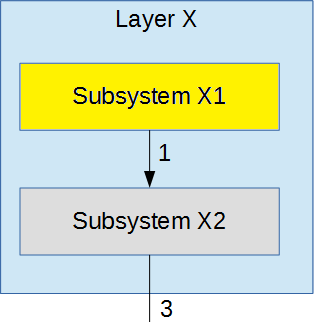
\includegraphics[width=0.60\textwidth]{images/subsystem}
 \caption{Example subsystem description diagram}
\end{figure}

\subsubsection{Subsystem Hardware}
The Web Layer will not consist of any hardware components for functionality purposes.

\subsubsection{Subsystem Operating System}
The main operating system (OS) for the overall app is Android OS.

\subsubsection{Subsystem Software Dependencies}
Any of the class files for Swift Scan will use Android's API along with Java SDK libraries for development of the GUI and back-end development of the functionality of the app, respectively.

\subsubsection{Subsystem Programming Languages}
The main programming language used for the Swift Scan app is Java and using Android's API for the GUI development.

\subsubsection{Subsystem Data Structures}
Swift Scan will contain two classes to write data to the internal text file and the second class will be used to retrieve the data and display the data to the user.  The second class where the data will be retrieved from the text file will have a method to sort the data as well so it can be displayed to the user.  In addition, the second class will also contain a method for updating any records within the text file, depending on what the user decides to update.

\subsubsection{Subsystem Data Processing}
A description of any algorithms or processing strategies that are worth discussing for the subsystem. If you are implementing a well-known algorithm, list it. If it is something unique to this project, discuss it in greater detail.
